% !Mode:: "TeX:UTF-8"
%!TEX program  = xelatex

\documentclass{cumcmthesis}
%\documentclass[withoutpreface,bwprint]{cumcmthesis} %去掉封面与编号页
\usepackage{float}
\usepackage{url}
\usepackage{enumitem}
\title{储油罐的变位识别与罐容表标定}
\tihao{A}
\baominghao{}
\schoolname{}
\membera{}
\memberb{}
\memberc{}
\supervisor{}
\yearinput{2018}
\monthinput{07}
\dayinput{29}

\begin{document}

 \maketitle
 \begin{abstract}


\keywords{}
\end{abstract}


\newpage

\section{问题重述}
    \subsection{问题背景}
    

    \subsection{问题提出}
    
    


\begin{figure}[H]
\begin{center}
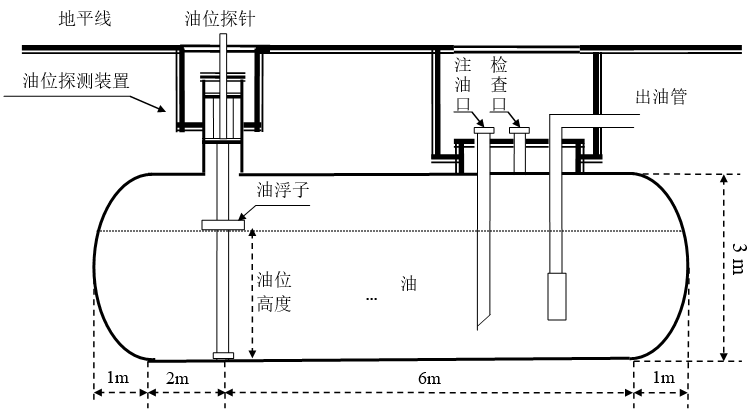
\includegraphics[scale=0.6]{figure1.png}
\caption{储油罐正面图}
\end{center}
\end{figure}

\begin{figure}[H]
\begin{center}
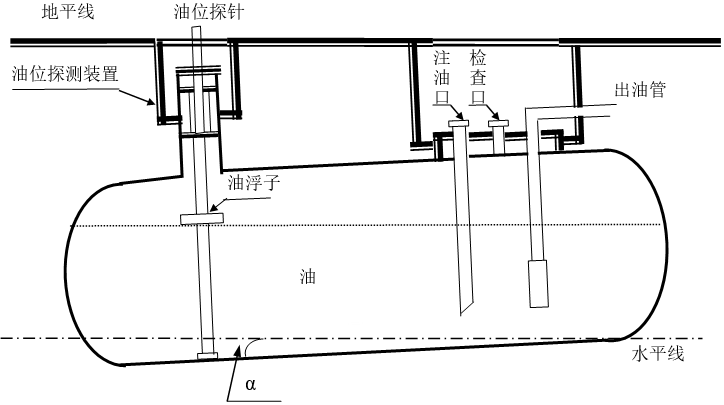
\includegraphics[scale=0.6]{figure2.png}
\caption{储油罐纵向倾斜变位后示意图}
\end{center}
\end{figure}

\begin{figure}[H]
\begin{center}
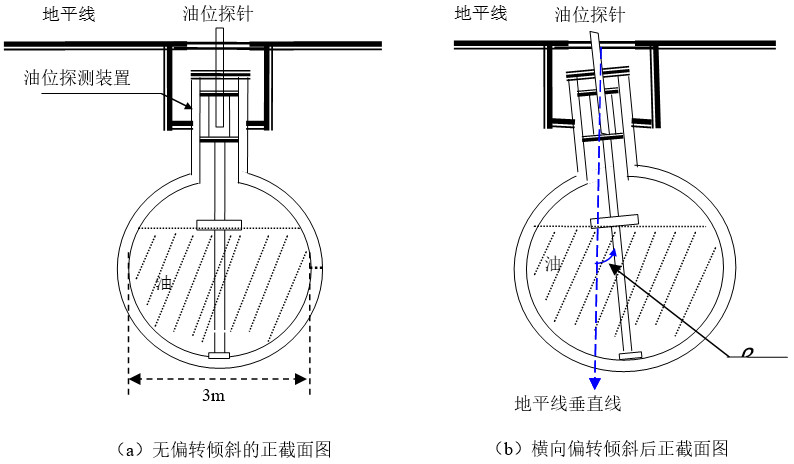
\includegraphics[scale=0.6]{figure3.png}
\caption{储油罐截面示意图}
\end{center}
\end{figure}

\begin{figure}[H]
\begin{center}
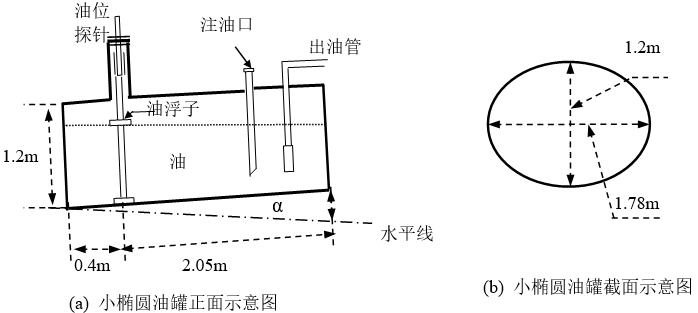
\includegraphics[scale=0.6]{figure4.png}
\caption{小椭圆型油罐形状及尺寸示意图}
\end{center}
\end{figure}

\section{问题分析}

\subsection{问题一分析}


\subsection{问题二分析}


\newpage

\section{模型的假设}


\section{模型的建立}

%\begin{equation}
%\begin{flushleft}
%\begin{aligned}
%S &= 1\\
%&= 2
%\end{aligned}
%\end{flushleft}
%\end{equation}

\begin{flalign*}
S(h) &= \frac{\pi ab}{2} + 2a(h-b)\sqrt{1 - \frac{1}{b^2}(b-h)^2}\\
     &\quad + sgn(h-b)\frac{b}{a}\left[\frac{1}{2}ab \arccos{\sqrt{1 - \frac{1}{b^2}(b-h)^2}} - \frac{a^2}{2b}\sqrt{1 - \frac{1}{b^2}(b-h)^2}(b-h)sgn(h-b) \right]
\end{flalign*}

%\section{符号说明}
%\begin{center}
%\begin{tabular}{cc}
% \hline
% \makebox[0.3\textwidth][c]{符号}	&  \makebox[0.4\textwidth][c]{意义} \\ \hline
% D	    & 木条宽度(cm) \\ \hline
% L	    & 木板长度(cm)  \\ \hline
% W	    & 木板宽度(cm)  \\ \hline
% N	    & 第n根木条  \\ \hline
% T	    & 木条根数  \\ \hline
%\end{tabular}
%\end{center}
%
%
%
%\section{绘制普通三线表格}
%表格应具有三线表格式,因此常用 booktabs宏包,其标准格式如表~\ref{tab001}~所示。
%\begin{table}[!htbp]
%\caption{标准三线表格}\label{tab001} \centering
%\begin{tabular}{ccccc}
%\toprule[1.5pt]
%$D$(in) & $P_u$(lbs) & $u_u$(in) & $\beta$ & $G_f$(psi.in)\\
%\midrule[1pt]
% 5 & 269.8 & 0.000674 & 1.79 & 0.04089\\
%10 & 421.0 & 0.001035 & 3.59 & 0.04089\\
%20 & 640.2 & 0.001565 & 7.18 & 0.04089\\
%\bottomrule[1.5pt]
%\end{tabular}
%\end{table}
%
%其绘制表格的代码及其说明如下。
%\begin{tcode}
%\begin{table}[!htbp]
%\caption[标签名]{中文标题}
%\begin{tabular}{cc...c}
%\toprule[1.5pt]
%表头第1个格   & 表头第2个格   & ... & 表头第n个格  \\
%\midrule[1pt]
%表中数据(1,1) & 表中数据(1,2) & ... & 表中数据(1,n)\\
%表中数据(2,1) & 表中数据(2,2) & ... & 表中数据(2,n)\\
%...................................................\\
%表中数据(m,1) & 表中数据(m,2) & ... & 表中数据(m,n)\\
%\bottomrule[1.5pt]
%\end{tabular}
%\end{table}
%\end{tcode}
%
%\bigskip
%table环境是一个将表格嵌入文本的浮动环境。
%tabular环境的必选参数由每列对应一个格式字符所组成:c表示居中,l表示左对齐,r表示右对齐,其总
%个数应与表的列数相同。此外,\verb|@{文本}|可以出现在任意两个上述的列格式之间,其中的文本将被插入每一行
%的同一位置。表格的各行以\verb|\\|分隔,同一行的各列则以\&分隔。
%\verb|\toprule|、\verb|\midrule|和\verb|\bottomrule|三个命令是由booktabs宏包提供的,其
%中\verb|\toprule|和\verb|\bottomrule|分别用来绘制表格的第一条(表格最顶部)和第三条(表格最底部)水平线,
%\verb|\midrule|用来绘制第二条(表头之下)水平线,且第一条和第三条水平线的线宽为1.5pt,第二条水平线的线宽为1pt。
%引用方法:“如表~\verb|\ref{标签名}|~所示”。
%
%
%参考文献
%\begin{thebibliography}{9}%宽度9
% \bibitem{bib:one} ....
% \bibitem{bib:two} ....
%\end{thebibliography}
%
%\newpage
%附录
%\appendix
%\section{排队算法--matlab 源程序}
%\begin{lstlisting}[language=matlab]
%kk=2;[mdd,ndd]=size(dd);
%while ~isempty(V)
%[tmpd,j]=min(W(i,V));tmpj=V(j);
%for k=2:ndd
%[tmp1,jj]=min(dd(1,k)+W(dd(2,k),V));
%tmp2=V(jj);tt(k-1,:)=[tmp1,tmp2,jj];
%end
%tmp=[tmpd,tmpj,j;tt];[tmp3,tmp4]=min(tmp(:,1));
%if tmp3==tmpd, ss(1:2,kk)=[i;tmp(tmp4,2)];
%else,tmp5=find(ss(:,tmp4)~=0);tmp6=length(tmp5);
%if dd(2,tmp4)==ss(tmp6,tmp4)
%ss(1:tmp6+1,kk)=[ss(tmp5,tmp4);tmp(tmp4,2)];
%else, ss(1:3,kk)=[i;dd(2,tmp4);tmp(tmp4,2)];
%end;end
%dd=[dd,[tmp3;tmp(tmp4,2)]];V(tmp(tmp4,3))=[];
%[mdd,ndd]=size(dd);kk=kk+1;
%end; S=ss; D=dd(1,:);
% \end{lstlisting}
% \section{规划解决程序--lingo源代码}
%\begin{lstlisting}[language=c]
%kk=2;
%[mdd,ndd]=size(dd);
%while ~isempty(V)
%    [tmpd,j]=min(W(i,V));tmpj=V(j);
%for k=2:ndd
%    [tmp1,jj]=min(dd(1,k)+W(dd(2,k),V));
%    tmp2=V(jj);tt(k-1,:)=[tmp1,tmp2,jj];
%end
%    tmp=[tmpd,tmpj,j;tt];[tmp3,tmp4]=min(tmp(:,1));
%if tmp3==tmpd, ss(1:2,kk)=[i;tmp(tmp4,2)];
%else,tmp5=find(ss(:,tmp4)~=0);tmp6=length(tmp5);
%if dd(2,tmp4)==ss(tmp6,tmp4)
%    ss(1:tmp6+1,kk)=[ss(tmp5,tmp4);tmp(tmp4,2)];
%else, ss(1:3,kk)=[i;dd(2,tmp4);tmp(tmp4,2)];
%end;
%end
%    dd=[dd,[tmp3;tmp(tmp4,2)]];V(tmp(tmp4,3))=[];
%    [mdd,ndd]=size(dd);
%    kk=kk+1;
%end;
%S=ss;
%D=dd(1,:);
% \end{lstlisting}


\end{document} 